\section{Implementation of a Local Integrated GEM-CSC Trigger for Phase-II Running}
\label{sec:slhc_algorithm_with_gems}

\subsection{The GEM proposal}

\textit{This text here is largely based on Michael Tytgat's introduction of the Conference Proceeding for his contribution in Zaragoza. It's fairly complete, but still too long. Aim for max 20 lines.}

Gas Electron Multipliers (GEMs) are gaseous, position sensitive devices featured by with extraordinary properties: spatial resolutions of order 100 $\mu$m, time resolutions of a few ns, detection efficiencies above 98\% and rate capabilities up to 10 MHz/cm$^2$. They can be operated in a stable manner in high radiation environments, at high gains exceeding $10^4$. %This makes GEMs very suitable detectors for a wide range of applications in many different fields including high energy particle physics. 

The present Muon System contains three different types of detectors for muon tracking and triggering CSCs, RPCs, and DTs. At present, the forward region with 1.6 $<|\eta|<$ 2.4 is only instrumented with CSCs, leaving this part of the detector less robust, with low redundancy for muon tracking and reconstruction. Furthermore, in the foward region one has a relatively high track density, and track projections in the bending plane are relatively short, which hampers the muon momentum determination and makes this area the most challenging region for muon detection. The main issue with respect to muon triggering in this region is the high background rate stemming from low-$p_T$ tracks that are misidentified as high-$p_T$ muons. Adding more detection layers with high granularity at high $|\eta|$ will yield additional space points for track reconstruction to be combined with the information from the CSCs. 

Triple-GEM based detectors are foreseen to be installed in the forward region (1.5 $<|\eta|<$ 2.4) of the muon system. This will improve both the muon momentum resolution and the background rejection at the trigger level, especially in the inner endcap stations where the muon track bending angle due to the magnetic field from the solenoid is largest. Pairs of triple-GEM chambers combined, or super-chambers, will be installed in the two inner endcap stations of the Muon System, as indicated in Fig.~\ref{fig:cms_upg_o_g_b_ni_gem_r_grid_130919}. In the current schedule, the inner endcap stations will be equiped with GEMs (GE1/1) during the second LHC Long Shutdown in 2017-2018, while the installation in the second endcap stations (GE2/1) will be done during the third LHC Long Shutdown scheduled beyond 2020. 

\begin{figure}[tb]
\begin{center}
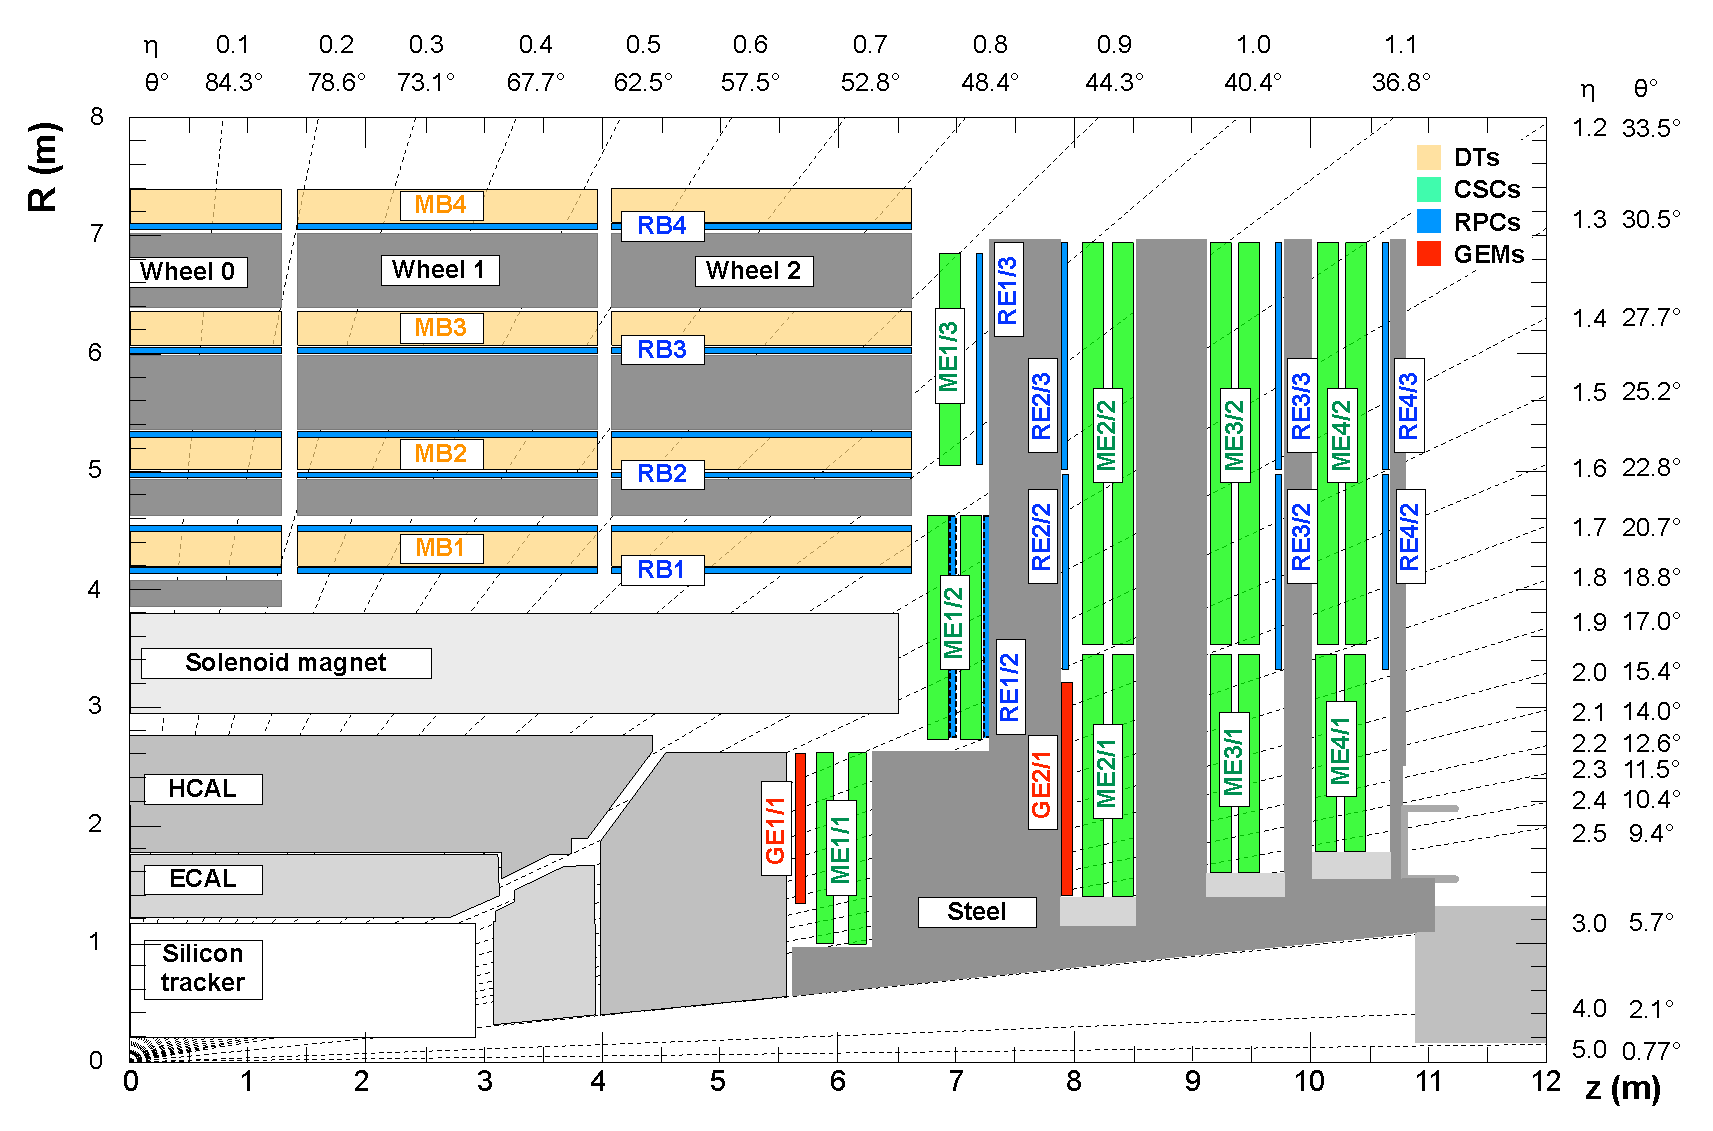
\includegraphics[width=0.9\textwidth]{figures/cms_upg_o_g_b_ni_gem_r_grid_130919.pdf}
\caption{Transverse section of the CMS detector with the foreseen locations of the GE1/1 and GE2/1 station.}
\label{fig:cms_upg_o_g_b_ni_gem_r_grid_130919}
\end{center}
\end{figure}

\subsection{Usage of GEM trigger primitives in the L1 CSC trigger}

\textit{This section is to show that we can use GEMs in the L1 CSC trigger and explain the options to modify the algorithm.}

GEM chambers have 384 strips. GEM digis will be combined in \textsc{OR}'ed combinations of $4$ strips, called GEM-CSC trigger GEM pads or simply pads. The very high efficiency ($>98\%$) results in a nearly $100\%$ efficiency to reconstruct a GEM pad in the first or second layer. This is clearly seen in Fig.~\ref{fig:gem_pad_eff_for_LCT_vs_phi_pt20_overlap}. 

\begin{figure}[htb]
\begin{center}
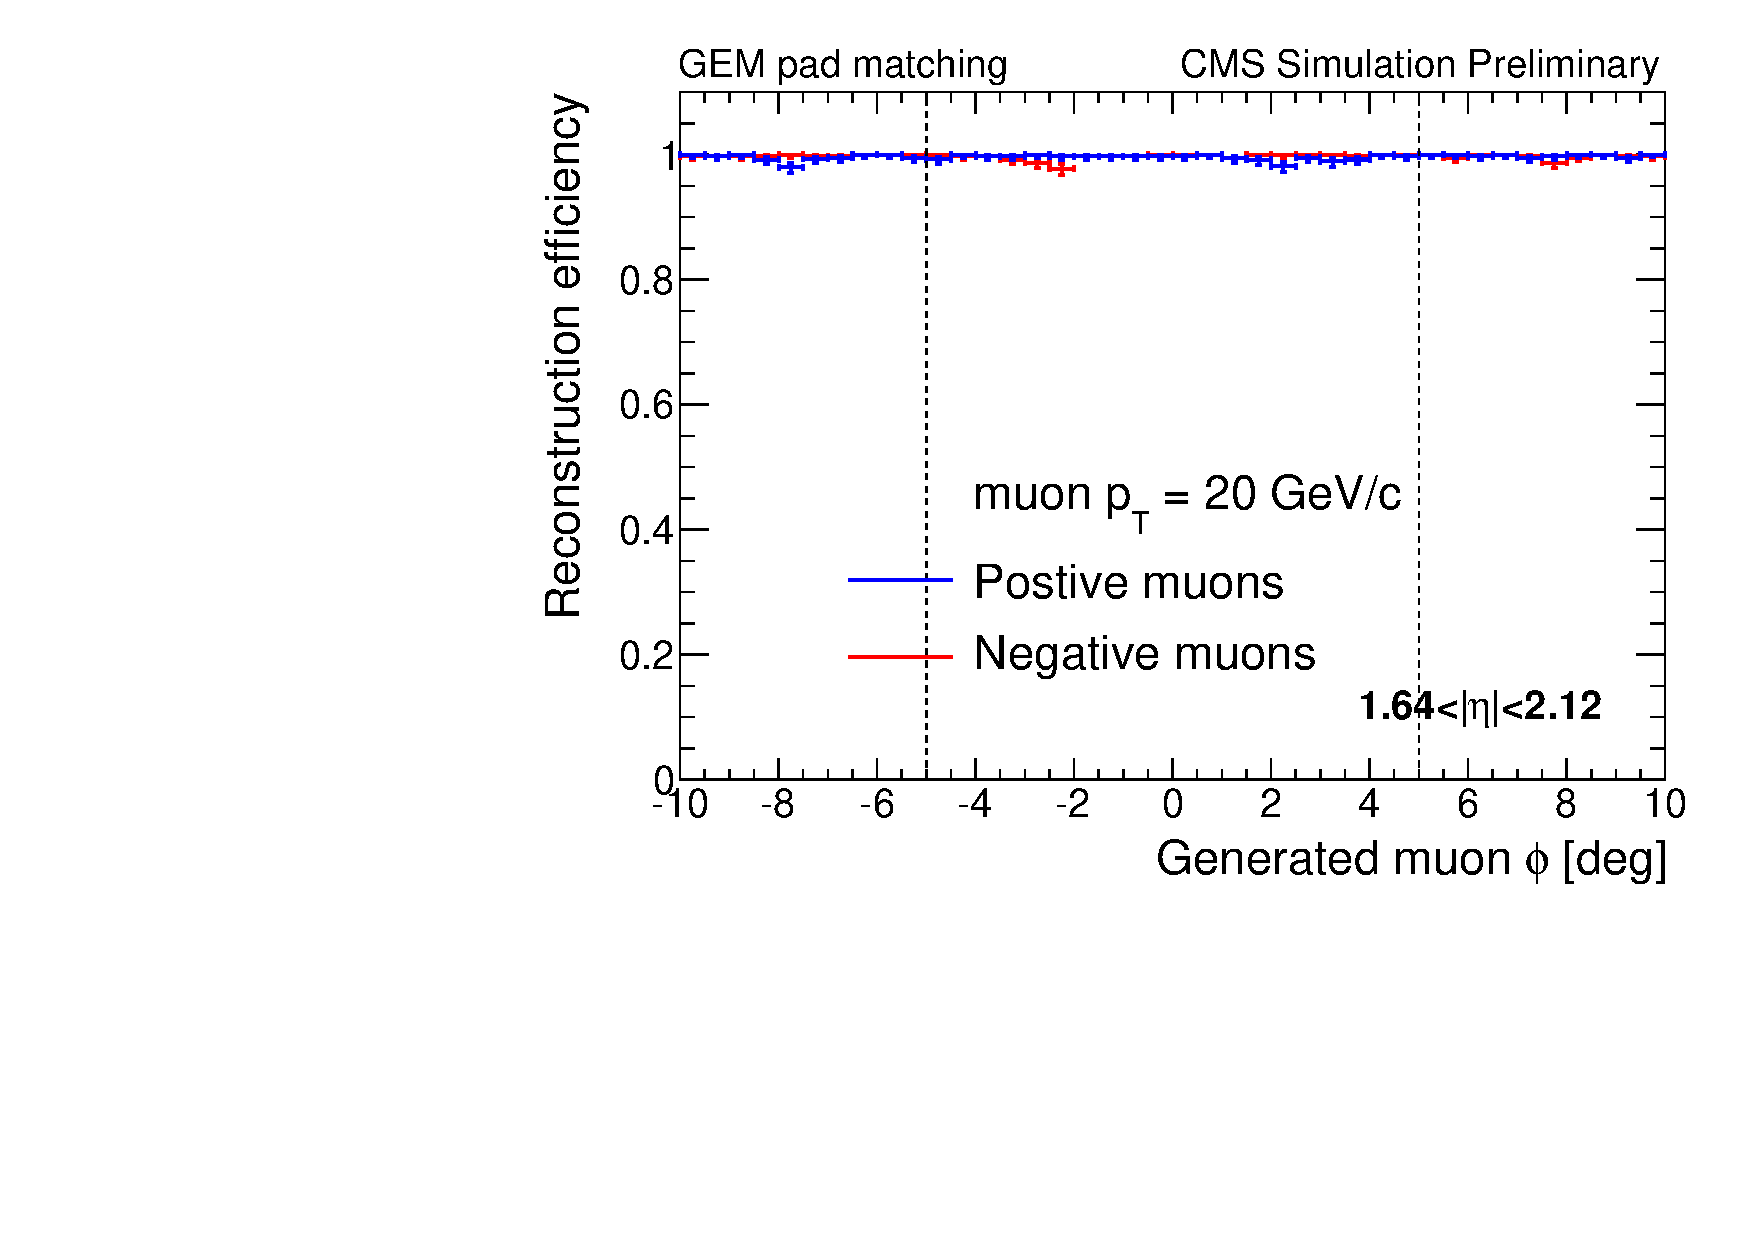
\includegraphics[width=0.5\textwidth]{figures/gem_pad_eff_for_LCT_vs_phi_pt20_overlap.pdf}
\caption{GEM pad reconstruction efficiency versus generated muon phi. The small dips are due to metal spacers in the GE1/1 prototype geometry. These spacers will not be present in the final geometry.}
\label{fig:gem_pad_eff_for_LCT_vs_phi_pt20_overlap}
\end{center}
\end{figure}

In what follows we will investigate several options to reduce the rate and increase the efficiency of the L1 CSC trigger. The first approach is to use the additional GEM information wherever possible in the present CSC trigger algorithm, e.g. to recover misreconstructed ALCTs or CLCTs, to improve the timing, to remove ghost stubs etc. This will be explained in \ref{subsec:slhc_algorithm_with_gems}. The second approach goes much beyond simlpy \textit{patching} up the CSC trigger. It includes reconstructing an LCT from a pair or triplet of ALCT, CLCT and GEM. In that sense a generalization of the definition of a stub in station 1 will be necessary. This will be explained in \ref{subsec:gem_csc_tmb_algorithm}.  
%\textit{Write down where pads are constructed in the hardware and how they are sent to the CSC TMB. Ask Gilles about the details}

\subsection{Factorized GEM-CSC TMB algorithm}
\label{subsec:slhc_algorithm_with_gems}

The factorized GEM-CSC TMB algorithm is aimed to improve the ALCT-to-CLCT matching algorithm and assign the bending angle to be used in the CSC Track Finder. 

The additional information can aid to reduce the rate and improve the efficiency in many ways. A frequent source of ineffiency is the loss of a low-hit ALCT(CLCT) in the CLCT-ALCT(ACLT-CLCT) matching. Whenever there is a GEM coincidence pad the timing of a CLCT(ALCT) can be corrected if necessary. In case a CLCT was missing, a GEM coincidence pad can be used to construct an LCT. In what follows we will investigate the possibility to patch up the CSC ME1/1 algorithm where it is necessary, so called the factorized GEM-CSC TMB algorithm. The other approach is to redesign the algorithm completely. 

\subsubsection{Reduction of soft stubs}
\label{subsubsec:reduction_of_soft_stubs}

As mentioned already in the introduction, a big issue to the present L1 CSC trigger is the flattening of the trigger rate at high $p_T^{cut}$. Low-$p_T$ muons are known to undergo multiple scattering in the iron yoke of the CMS endcap. This scattering causes the stubs to become aligned. As a result, the CSC Track-Finder will see a straight track for the low-$p_T$ muon and will assign a much higher transverse momumentum. If one is able to prevent the soft stubs in station 1 to be used in the track-fit, it will be less likely that a soft muon is given a high $p_T$. 

With the installation of double-layered GEM chambers in station 1, measurement of the bending angle becomes possible. \textit{Add a figure here about the geometrical setup of the bending angle.} Fig.~\ref{fig:GEMCSCdPhi_chambers_reverse} shows the GE1/1-ME1/1 bending angle of 5 GeV and 20 GeV muons in even and odd chambers. The odd chambers show a larger separation of the muons since they are spaced farther apart along the beamline.

\begin{figure}[htb]
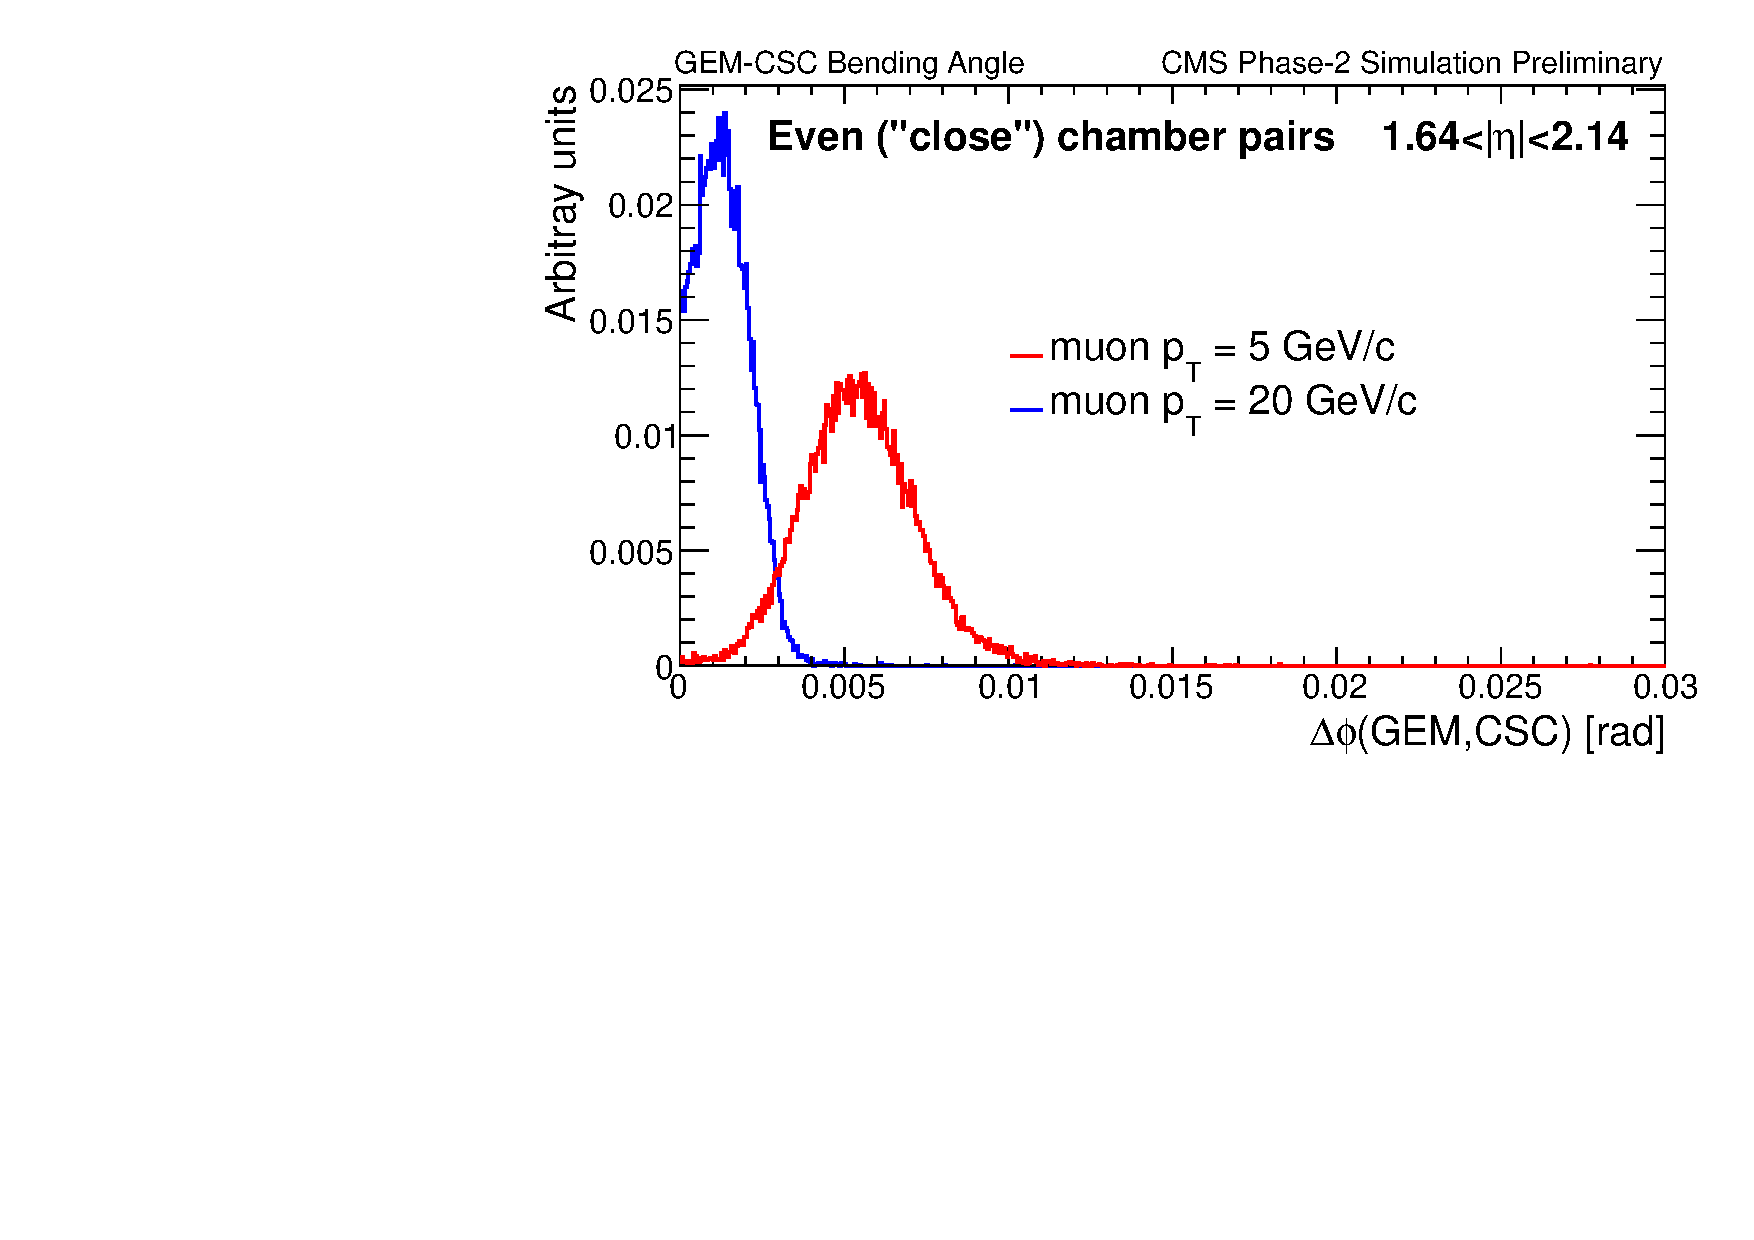
\includegraphics[width=0.5\textwidth]{figures/GEMCSCdPhi_even_chambers_reverse.pdf}
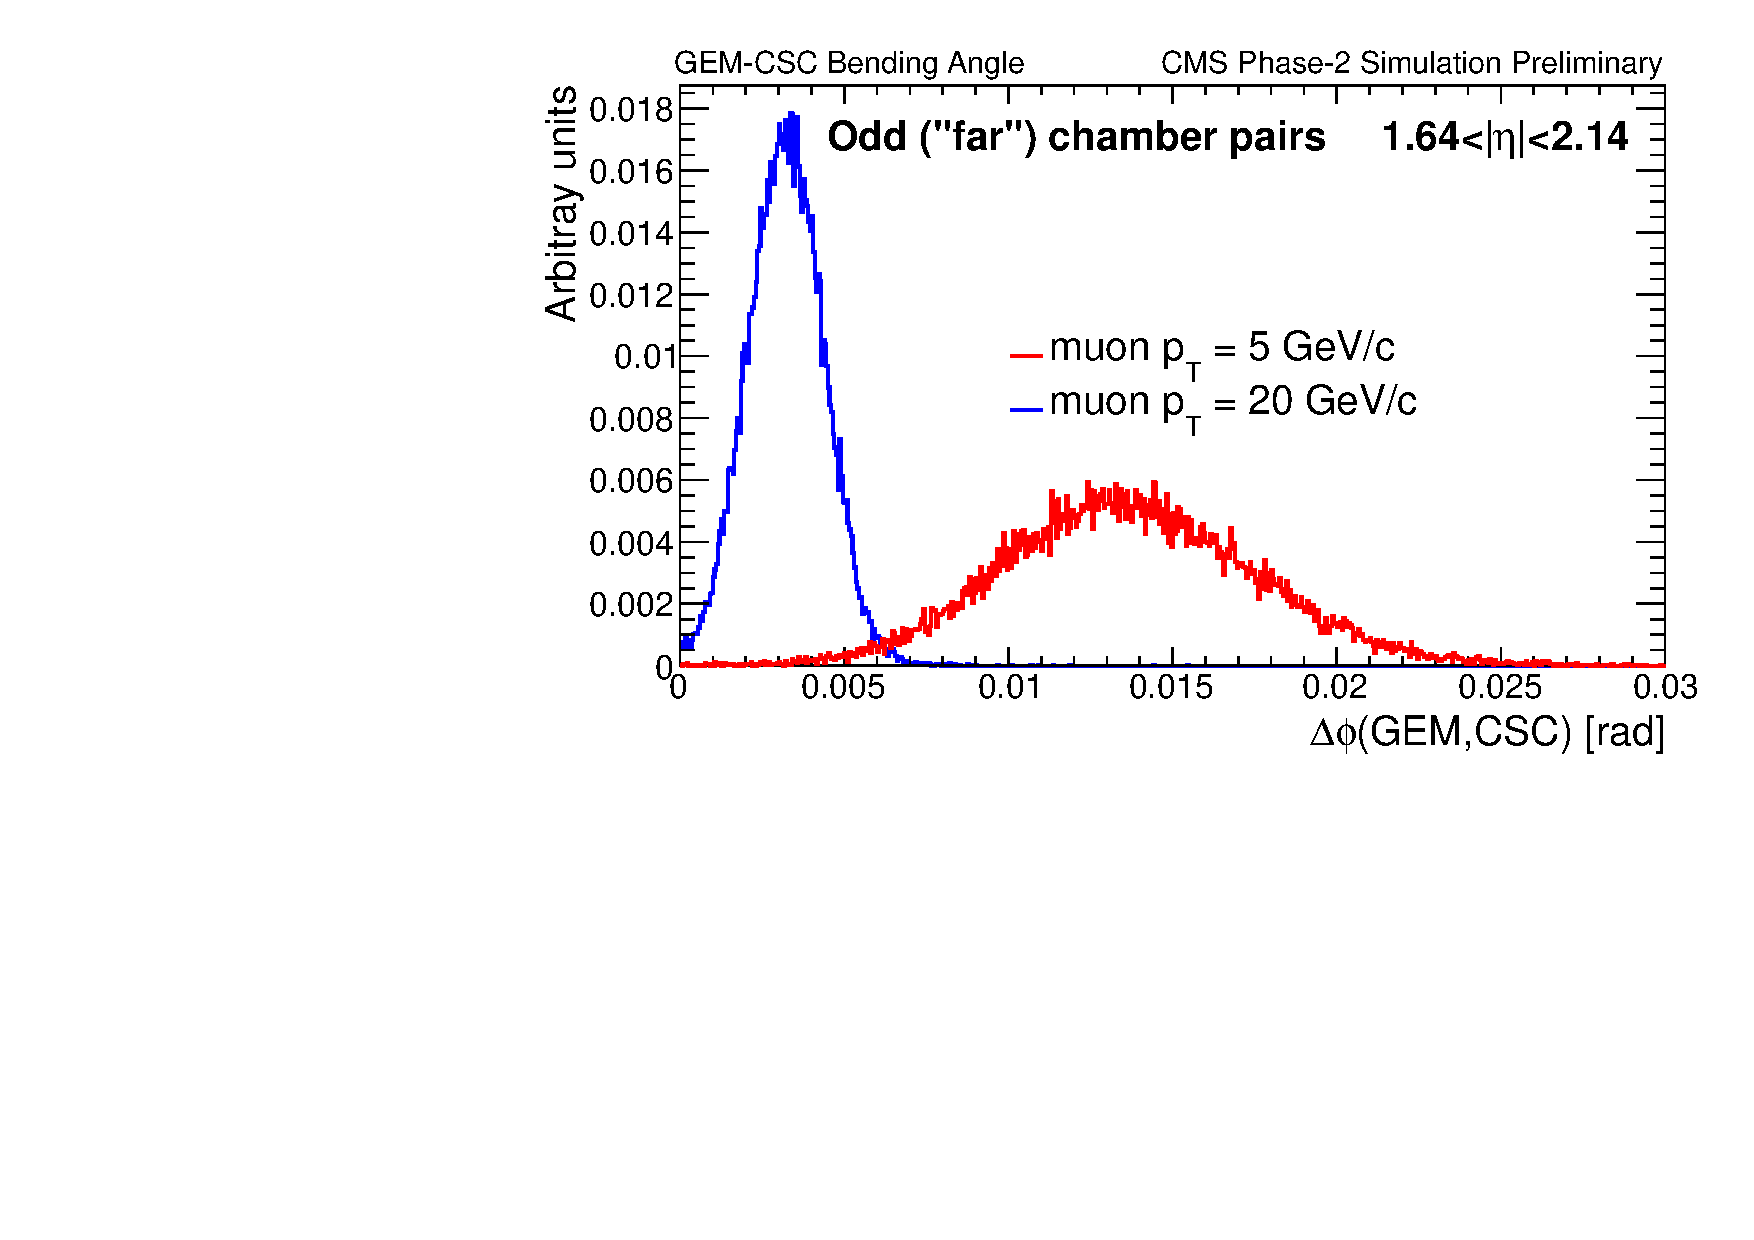
\includegraphics[width=0.5\textwidth]{figures/GEMCSCdPhi_odd_chambers_reverse.pdf}
\caption{Comparison of GEM-CSC bending angle for muons with low pt and high pt for even (left) and odd (right) numbered chambers.}
\label{fig:GEMCSCdPhi_chambers_reverse}
\end{figure}

The discrimination power can now applied in the L1 CSC trigger algorithm. Once the LCTs are reconstructed from an ALCT-CLCT pair via ALCT or CLCT-centric matching, we can try to assign a GEM bending angle to it. First, all GEM trigger pads are collected within the bunch crossing range [5,7], or +1/-1 about the central bunch crossing for a particular LCT. The default value for GEM-CSC bending angle is $-99$. If at least 1 GEM trigger pad is available (SPECFICY), the bending angle is assigned $+99$. To consider a GEM pad as \textit{matched} it has to be within specified \texttt{delta\_eta} and \texttt{delta\_phi} ranges. If there are multiple ones, only the $\min|delta_phi|$ is considered as matched. The unmatched LCTs can be kept or removed. 

To illustrate the effect of this simple pad matching procedure, we ran the modified L1 CSC trigger algorithm for various bending angles corresponding with muon transverse momenta of 5, 6, 10, 15, 20, 30 and 40 GeV. Unmatched LCTs were removed from the event and were not used in the track-fit and Global Muon Trigger. The resulting trigger rate vs $p_T^\text{cut}$ and $\eta$ was calculated by combining the samples. The result is shown in in Fig.~\ref{fig:l1_trigger_rate_csc_gem}. 

\begin{figure}[htb]
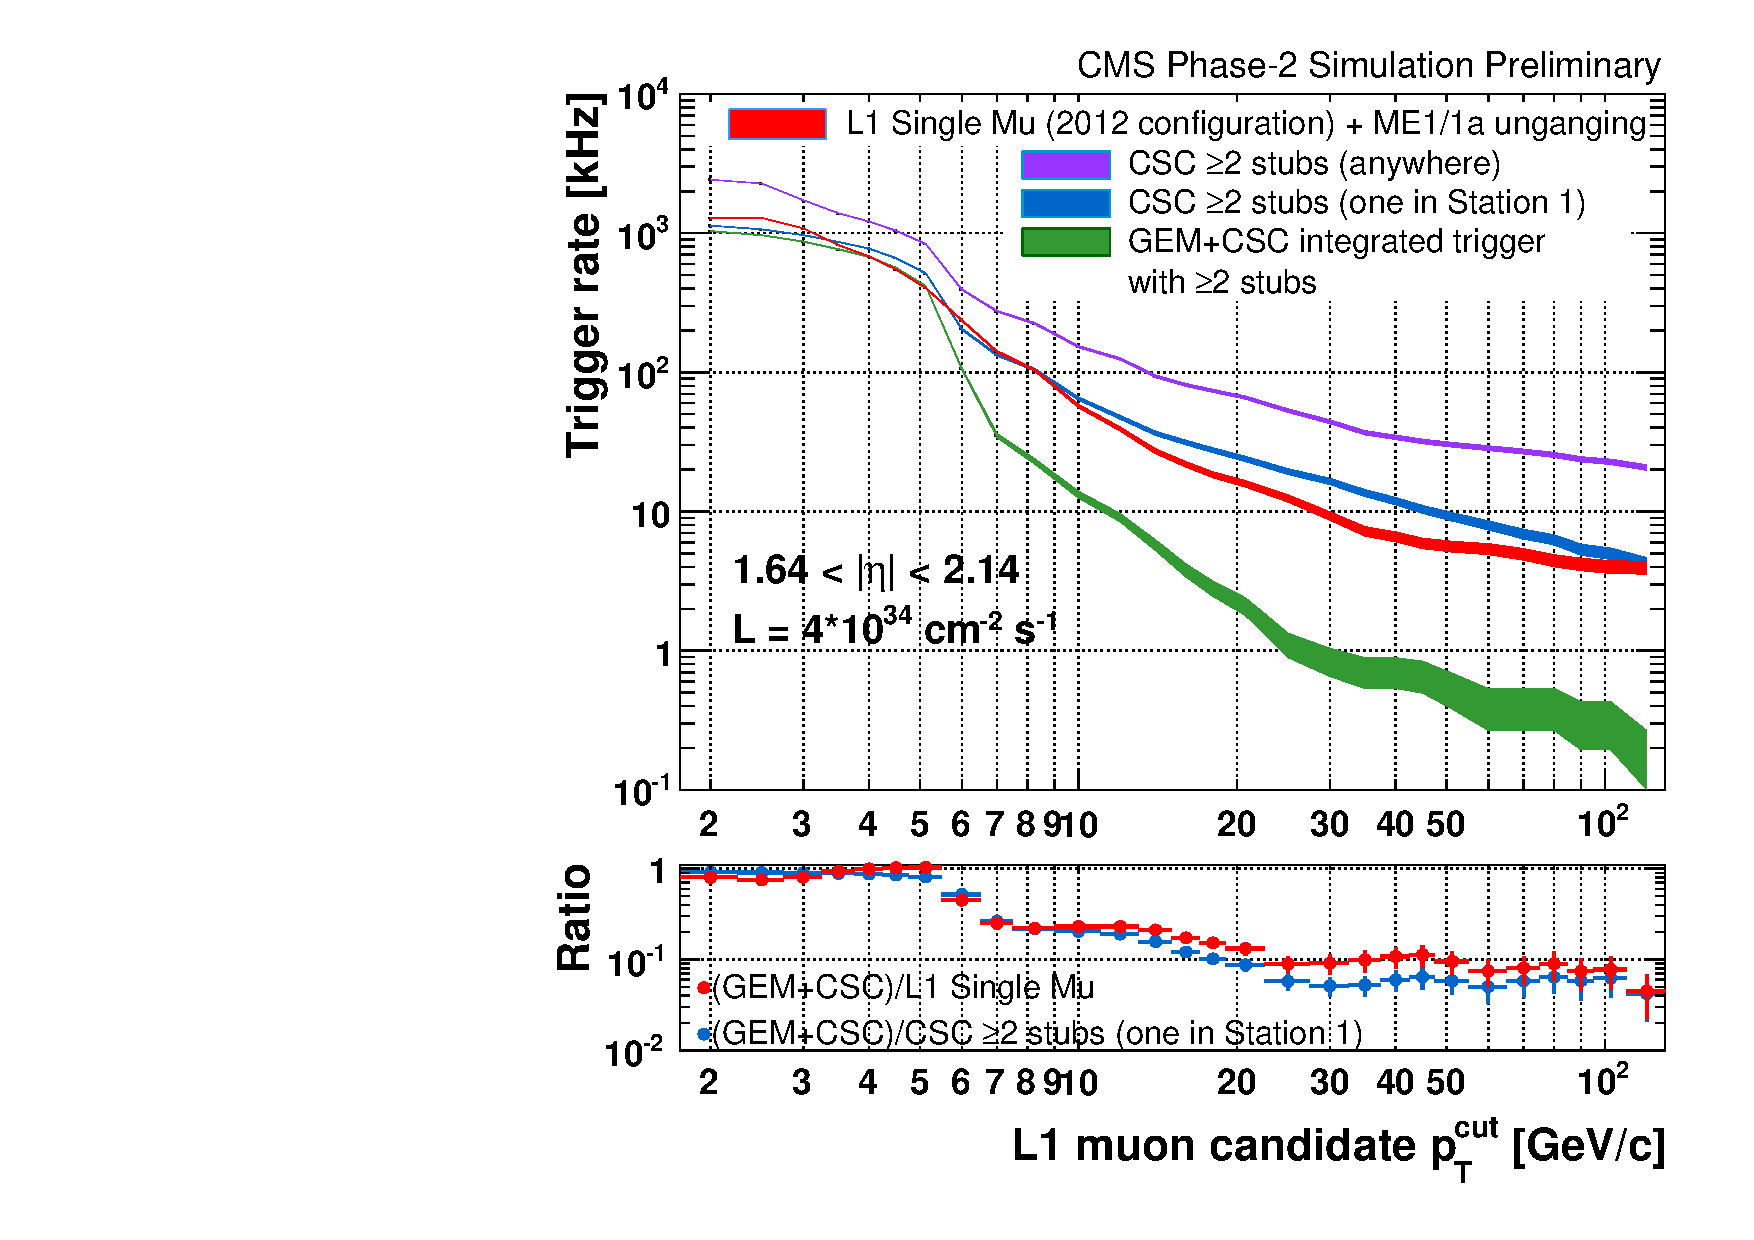
\includegraphics[width=0.5\textwidth]{figures/rates_vs_pt__PU100__def_2s_2s1b_2s1bgem__loose.pdf}
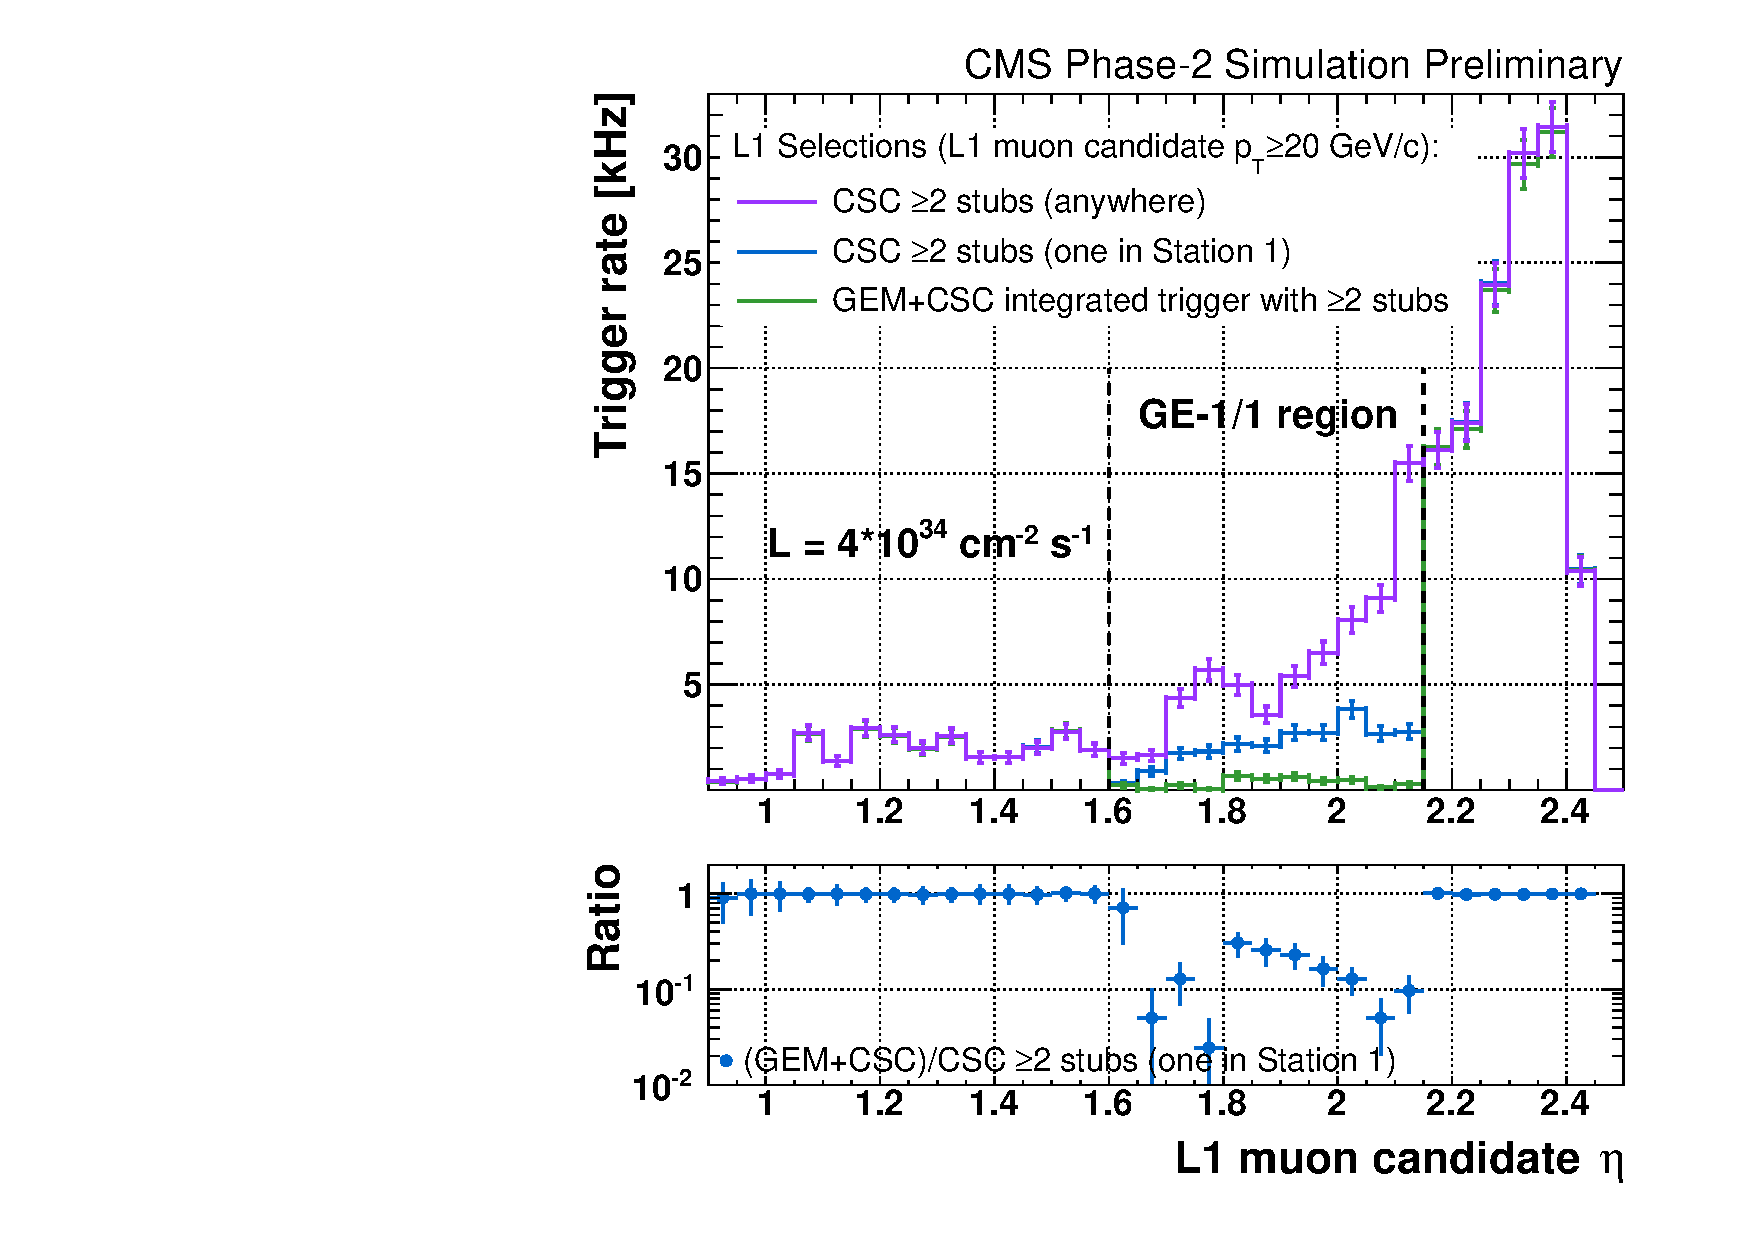
\includegraphics[width=0.5\textwidth]{figures/rates_vs_eta__minpt20__PU100__def_2s_2s1b_2s1bgem.pdf}
\caption{Comparison of the trigger rates (left vs $p_T^\text{cut}$, right vs muon  $\eta$) for the Global Muon Trigger in the 2012 configuration with the CSC Track-Finder track rates for at least 2 stubs (loose), at least 2 stubs with at least one 1 stub from ME1/b (medium), and at least one 2 stubs with at least one 1 stub from ME1/b and a GEM pad (tight). The CSC TF used all patterns. The bottom plot shows the ratio of tight/GMT and tight/medium.}
\label{fig:l1_trigger_rate_csc_gem}
\end{figure}

%\subsubsection{Assignment of the bending angle}
%
%\textit{This is the algorithm as it is currently in software. In firmware there will be no simtrack information and it will be somewhat simpler.}
%
%After the LCTs are reconstructed in the matching step, they can be matched to LCTs. First a check is done if there are any good LCTs at all in the bunch crossing window that is considered. If there are no valid LCTs, no assignment is done. The algorithm will then proceed with a triple-nested loop: on all bunch crossings, on all potential LCT pairs in this bunch crossing, and both LCTs in the pair. 
%
%For each LCT it will start by setting the bending angle to the value $-99$, which is the default value. The CSC trigger geometry is enabled to calculate the position of the LCT int the first CSC layer in the global CMS coordinate system. If the global $\eta$ does not pass the GEM fiduciality requirement, no matching is done. If it does pass the requirement, the bending angle is set to $+99$. The algorithm then proceeds with looping on all trigger pads. For each trigger pad, the global position in the CMS coordinate system is calculated. The bending angle, $\Delta\phi_\text{GEM,CSC}$, is then calculated as $\text{abs}(\phi_\text{GEM}-\phi_\text{CSC})$. The $\Delta\eta$ is calculated from the global position as $\text{abs}(\eta_\text{GEM}-\eta_\text{CSC})$. If $\Delta\eta$ is smaller than the currently fixed value of $0.08$, if  $\Delta\phi_\text{GEM,CSC}$ value is smaller than the $\Delta\phi_\text{GEM,CSC}$ expected for this muon track, and the to now calculated minimum the bending angle is stored in the dataformat. Using a look-up-table the bending angle is converted to a bit-wise value. 

\subsubsection{Low-hit stub recovery in ALCT-CLCT matching}

\textit{First part of this subsection is about ALCT-CLCT. Second part are the results for CLCT-ALCT.}

A frequent source of inefficiency is when insufficient strip layers were hit within 4 BX to form a CLCT. The current conditions for a CLCT to pass the pre-trigger and trigger requirement are 3/6 and 4/6 respectively. On the one hand, one can reduce the trigger requirement of 4/6 to 3/6 layers. One the other hand, the introduction of a double-layered GEM system effectively increases the number of layers from 6 to 8. The CLCT reconstruction efficiency should go up if we require 4/8 instead of 4/6 layers. The results of this are show in Fig. for two different high pile-up scenarios.

\textit{Make two plots: PU140 and PU400 for fixed pre-trigger of 3 and trigger of 3/6, 4/6 and 4/8} 

\begin{figure}[htb]
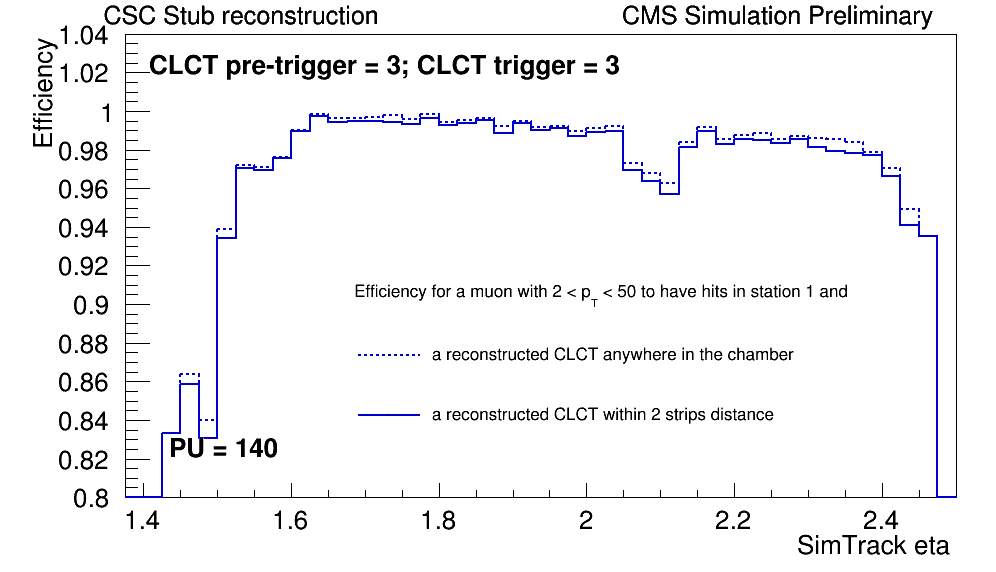
\includegraphics[width=0.5\textwidth]{figures/simTrackToClctMatchingEfficiencyVsEtaME1_pu140_preTrig33.png}
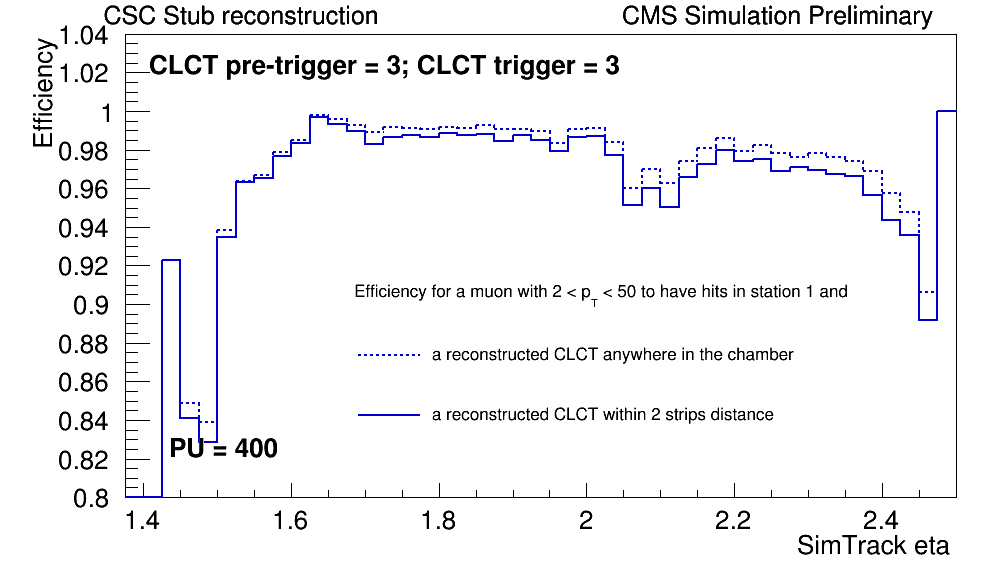
\includegraphics[width=0.5\textwidth]{figures/simTrackToClctMatchingEfficiencyVsEtaME1_pu400_preTrig33.png}
\caption{CLCT reconstruction efficiency for a pre-trigger and trigger requirement of 3 for several pile-up scenarios.}
\label{fig:clct_reconstruction_efficiency_eta_trig_pu}
\end{figure}

\textit{Add here the plots for CLCT-ALCT matching.}

\subsubsection{Disambiguation of best and second best stub}

\subsubsection{Substitution of a GEM for an ALCT/CLCT in the matching}

As explained in section (REFERENCE) the upper and lower part of the ME1/1 chamber, called ME1/b and ME1/a respectively have a separate CFEBs to process the comparator digis. This has far-reaching consequences, in particular for muons going through the overlap region or through the edges of the chamber. If a muon goes through the overlap region, it may have hit at least 4 layers hit in the whole ME1/1 chamber, but may not have enough hits in either sub-chamber to pass the pre-trigger and trigger requirement. An example is the case: 3 layers hit in ME1/b and 2 layers hit in ME1/a. 

In case the other ME1/1 stub was not reconstructed, one can make an attempt to form an LCT out of the available ME1/1 stub and a GEM coincidence pad.

\textit{Construction of coincidence pads in the TMB. Make a separate section or not?}

%\subsubsection{Construction of GEM coincidence pads}

T
After the ALCTs and CLCTs are retrieved from the corresponding processors, the GEM pads from the neighbouring GE1/1 chambers are collected. The GEM pads will be assigned a chamber number, a roll number, a pad number and a bunch crossing. The current definition of a coincidence pad is as follows:
\begin{itemize}
\item Pad 1 comes from chamber 1
\item Pad 2 comes from chamber 2
\item Both pads have the same pad number
\item Both pads have the same eta partition number
\item The time of pad 1 and pad2 can differ by at most 1 bunch crossing
\end{itemize}


Suppose that in the ALCT centric matching no good CLCT was found within the bunch crossing window, one can use substitute a GEM coincidence pad, provided it was found, for a CLCT. This requires a more general definition of an LCT.  

%\textit{Go in more details about the definition of a GEM pad}
%
%Of course, the current definition is subject to improvement to allow for various cases that can still be regarded as a coincidence pad. For instance, a muon hitting a GEM on the edge of two eta partitions in the first chamber could hit the eta partition above below (depending how it was going. A second case is where a muon hit a GEM chamber on the edge of certain pad in the first chamber. In this case it could go through a pad with a pad higher or lower number in the second chamber. In the future one could go for an extended definition more extended version of a GEM pad to allow for such cases.  

%\subsubsection{Wrapping of pads and co-pads}
%
%\textit{Figure out how the GEM pads are encoded in the data. Maybe it does not have to be done in firmware.}



\subsubsection{Correction of stub timing}





\subsection{Future algorithm with additional improvements}

The following is an overview of the algorithm 

\begin{enumerate}
\item Retrieve the ALCTs from the ALCT processor board
\item Reconstruct the CLCTs in the CLCT processor board for ME1/b
\item Reconstruct the CLCTs in the CLCT processor board for ME1/a
\item Stub matching procedure.
\begin{itemize}
\item CLCT-to-ALCT matching
\item ALCT-to-CLCT matching
\begin{enumerate}
\item For each bunch crossing in the maximum number of ALCT BXs check if the ALCT has a valid pattern
\item Check if there are any trigger pads and co-pads
\item For each CLCT in the CLCT matching BX window, check if the CLCT has a valid pattern
\item If the CLCT has less than 4 layers hit and if there was no trigger pad, continue with the next CLCT. 
\item Correlate the best CLCT with the best ALCT and the second best CLCT with the second best ALCT.
\end{enumerate}
\end{itemize}
\item Assignment of the GEM-CSC bending angle. 
\item Reduction of the number of LCTs 
\end{enumerate}

\subsubsection{GEM-CSC TMB algorithm}
\label{subsec:gem_csc_tmb_algorithm}

The second option goes beyond patching up the existing improved ME1/1 algorithm. In this algorithm we consider the ALCT, CLCT and GEM and perform a sort of voting to construct a more general LCT with 3 different LCT classes
\begin{itemize}
\item ALCT and CLCT
\item ALCT and GEM
\item CLCT and GEM
\end{itemize}
In case one has ALCT, CLCT and GEM, only the two highest quality stubs are chosen to reconstruct the LCT. Evidently, this change in object definition goes together with a change in dataformat. 

\subsubsection{Future possibilities for GEM-CSC triggering}
\label{subsec:future_possibilities_for_gem_csc_triggering}

\textit{Write something here about GE2/1-ME2/1 trigger options}

\textit{Write something here about ME0 trigger options}

\newpage
